%\documentclass[UTF8]{ctexart} % use larger type; default would be 10pt
\documentclass[a4paper]{article}
\usepackage{xeCJK}
%\usepackage[utf8]{inputenc} % set input encoding (not needed with XeLaTeX)

%%% Examples of Article customizations
% These packages are optional, depending whether you want the features they provide.
% See the LaTeX Companion or other references for full information.

%%% PAGE DIMENSIONS
\usepackage{geometry} % to change the page dimensions
\geometry{a4paper} % or letterpaper (US) or a5paper or....
\geometry{margin=1in} % for example, change the margins to 2 inches all round
% \geometry{landscape} % set up the page for landscape
%   read geometry.pdf for detailed page layout information

\usepackage{graphicx} % support the \includegraphics command and options

% \usepackage[parfill]{parskip} % Activate to begin paragraphs with an empty line rather than an indent

%%% PACKAGES
\usepackage{booktabs} % for much better looking tables
\usepackage{array} % for better arrays (eg matrices) in maths
\usepackage{paralist} % very flexible & customisable lists (eg. enumerate/itemize, etc.)
\usepackage{verbatim} % adds environment for commenting out blocks of text & for better verbatim
\usepackage{subfig} % make it possible to include more than one captioned figure/table in a single float
% These packages are all incorporated in the memoir class to one degree or another...

%%% HEADERS & FOOTERS
\usepackage{fancyhdr} % This should be set AFTER setting up the page geometry
\pagestyle{fancy} % options: empty , plain , fancy
\renewcommand{\headrulewidth}{0pt} % customise the layout...
\lhead{}\chead{}\rhead{}
\lfoot{}\cfoot{\thepage}\rfoot{}

%%% SECTION TITLE APPEARANCE
\usepackage{sectsty}
\allsectionsfont{\sffamily\mdseries\upshape} % (See the fntguide.pdf for font help)
% (This matches ConTeXt defaults)

%%% ToC (table of contents) APPEARANCE
\usepackage[nottoc,notlof,notlot]{tocbibind} % Put the bibliography in the ToC
\usepackage[titles,subfigure]{tocloft} % Alter the style of the Table of Contents
\renewcommand{\cftsecfont}{\rmfamily\mdseries\upshape}
\renewcommand{\cftsecpagefont}{\rmfamily\mdseries\upshape} % No bold!

%%% END Article customizations

%%% The "real" document content comes below...

\setlength{\parindent}{0pt}
\usepackage{physics}
\usepackage{amsmath}
%\usepackage{symbols}
\usepackage{AMSFonts}
\usepackage{bm}
%\usepackage{eucal}
\usepackage{mathrsfs}
\usepackage{amssymb}
\usepackage{float}
\usepackage{multicol}
\usepackage{abstract}
\usepackage{empheq}
\usepackage{extarrows}
\usepackage{textcomp}
\usepackage{fontspec}
\usepackage{braket}
\usepackage{siunitx}
\sisetup{
	separate-uncertainty = true,
	inter-unit-product = \ensuremath{{}\cdot{}}
}
\usepackage{mhchem}
\usepackage{hyperref}
\hypersetup{
	colorlinks=true,
	linkcolor=black,
	filecolor=magenta,      
	urlcolor=cyan,
}

\DeclareMathOperator{\p}{\prime}
\DeclareMathOperator{\ti}{\times}
\DeclareMathOperator{\intinf}{\int_0^\infty}
\DeclareMathOperator{\intdinf}{\int_{-\infty}^\infty}
\DeclareMathOperator{\intzpi}{\int_0^\pi}
\DeclareMathOperator{\intztpi}{\int_0^{2\pi}}
\DeclareMathOperator{\sumninf}{\sum_{n=1}^{\infty}}
\DeclareMathOperator{\sumninfz}{\sum_{n=0}^\infty}
\DeclareMathOperator{\sumiinf}{\sum_{i=1}^{\infty}}
\DeclareMathOperator{\sumiinfz}{\sum_{i=0}^\infty}
\DeclareMathOperator{\sumkinf}{\sum_{k=1}^{\infty}}
\DeclareMathOperator{\sumkinfz}{\sum_{k=0}^\infty}
\DeclareMathOperator{\e}{\mathrm{e}}
\DeclareMathOperator{\I}{\mathrm{i}}
\DeclareMathOperator{\Arg}{\mathrm{Arg}}
\DeclareMathOperator{\ra}{\rightarrow}
\DeclareMathOperator{\llra}{\longleftrightarrow}
\DeclareMathOperator{\lra}{\longrightarrow}
\DeclareMathOperator{\dlra}{\Leftrightarrow}
\DeclareMathOperator{\dra}{\Rightarrow}
\newcommand{\bkk}[1]{\Braket{#1|#1}}
\newcommand{\bk}[2]{\Braket{#1|#2}}
\newcommand{\bkev}[2]{\Braket{#2|#1|#2}}



\DeclareMathOperator{\hV}{\hat{\vb{V}}}

\DeclareMathOperator{\hx}{\hat{\vb{x}}}
\DeclareMathOperator{\hy}{\hat{\vb{y}}}
\DeclareMathOperator{\hz}{\hat{\vb{z}}}

\DeclareMathOperator{\hA}{\hat{\vb{A}}}

\DeclareMathOperator{\hQ}{\hat{\vb{Q}}}
\DeclareMathOperator{\hI}{\hat{\vb{I}}}
\DeclareMathOperator{\psis}{\psi^\ast}
\DeclareMathOperator{\Psis}{\Psi^\ast}
\DeclareMathOperator{\hi}{\hat{\vb{i}}}
\DeclareMathOperator{\hj}{\hat{\vb{j}}}
\DeclareMathOperator{\hk}{\hat{\vb{k}}}
\DeclareMathOperator{\hr}{\hat{\vb{r}}}
\DeclareMathOperator{\hT}{\hat{\vb{T}}}
\DeclareMathOperator{\hH}{\hat{H}}
\DeclareMathOperator{\hh}{\hat{h}}               % helicity
\DeclareMathOperator{\hL}{\hat{\vb{L}}}
\DeclareMathOperator{\hp}{\hat{\vb{p}}}

\DeclareMathOperator{\ha}{\hat{\vb{a}}}
\DeclareMathOperator{\hS}{\hat{\vb{S}}}
\DeclareMathOperator{\hSigma}{\hat{\bm\Sigma}}
\DeclareMathOperator{\hJ}{\hat{\vb{J}}}
\DeclareMathOperator{\hP}{\hat{\vb{P}}}          % Parity
\DeclareMathOperator{\hC}{\hat{\vb{C}}} 
\DeclareMathOperator{\Tdv}{-\dfrac{\hbar^2}{2m}\dv[2]{x}}
\DeclareMathOperator{\Tna}{-\dfrac{\hbar^2}{2m}\nabla^2}
\DeclareMathOperator{\vna}{\vnabla}
\DeclareMathOperator{\nna}{\nabla^2}
\newcommand{\naCarExpd}[1]{\pdv[2]{#1}{x} + \pdv[2]{#1}{y} + \pdv[2]{#1}{z}}
\newcommand{\naCyl}{\qty[\dfrac{1}{\rho}\pdv{\rho}\qty(\rho\pdv{\rho}) + \dfrac{1}{\rho^2}\pdv[2]{\phi} + \pdv[2]{z}]}

%\DeclareMathOperator{\g#0}{\gamma^0}
%\DeclareMathOperator{\g1}{\gamma^1}
%\DeclareMathOperator{\g2}{\gamma^2}
%\DeclareMathOperator{\g3}{\gamma^3}
%\DeclareMathOperator{\g5}{\gamma^5}
\newcommand{\g}[1]{\gamma^{#1}}
\DeclareMathOperator{\gmuu}{\gamma^\mu}
\DeclareMathOperator{\gmud}{\gamma_\mu}
%\newcommand{\G}[2]{g^{#1#2}}

\newcommand{\subsbul}{\subsection*{$ \bullet $}}
\newcommand{\ex}[1]{\paragraph{13-#1}}
\newcommand{\subex}[1]{\subparagraph{#1}}
\newcommand{\dis}{\displaystyle}
\newcommand{\iden}{{\large \bm{1}}}
\newcommand{\qed}{$ \Square $}
\newcommand{\tPhi}{\tilde{\Phi} }
\DeclareMathOperator{\au}{\mathrm{a.u.}}

\numberwithin{equation}{section}
%\setcounter{secnumdepth}{4}
\setcounter{tocdepth}{4}
%\allowdisplaybreaks[4]

\usepackage{xcolor}
\definecolor{codegray}{gray}{0.9}
\newfontfamily\Consolas{Consolas}
\newcommand{\code}[1]{\colorbox{codegray}{{\Consolas#1}}}

\title{\textbf{Advanced Physical Chemistry II}\\HW}
\author{王石嵘
\vspace{5pt}\\
161240065\\
%Email: shirong\_wang@berkeley.edu
}
\date{\today} % Activate to display a given date or no date (if empty),
         % otherwise the current date is printed 

\begin{document}
% \boldmath

\maketitle

%\tableofcontents

%\newpage

\setcounter{section}{12}
\section{Molecular Spectroscopy}
3, 7, 14, 18, 24, 28, 32, 37, 40, 43, 45, 51\\
\ex{3}
\begin{equation}\label{key}
\mu = \dfrac{1.01 \cross 126.9}{1.01 + 126.9}\cross \num{1823}\au = \num{1.827e3}\au
\end{equation}
\begin{align}\label{key}
\tilde{B} &= \dfrac{\hbar}{4\pi c\mu R_e^2} = \dfrac{1}{4\pi\cross 137 \cross \num{1.827e3}}\au \cross\dfrac{1}{(\SI{160.4}{pm})^2}\notag\\
&= \SI{1.682e-5}{pm}\cross\dfrac{1}{(\SI{160.4}{pm})^2}\notag\\
&= \SI{6.54}{cm^{-1}}
\end{align}
\begin{align}
c\tilde{B} = \SI{3e8}{m.Hz}\cross\SI{6.54e2}{m^{-1}} = \SI{1.96e5}{MHz}
\end{align}
\ex{7}
\begin{equation}\label{key}
\mu = \dfrac{38.96\cross 34.97}{38.96 + 34.97}\si{amu} = \SI{18.44}{amu} = \SI{3.06e-26}{kg}
\end{equation}
\begin{equation}\label{key}
k = \mu(2\pi c \tilde{\nu})^2 = \num{3.06e-26} (2\pi \cross\num{3e8}\cross 27800)^2 = \SI{84.0}{N.m}
\end{equation}
\begin{equation}\label{key}
T = \dfrac{1}{c\tilde{\nu}} = \dfrac{1}{\num{3e8}\cross 27800} = \SI{1.20e-13}{s}
\end{equation}
\ex{14}
\begin{align}
R(0) &= \tilde{\nu} + 2\tilde{B}_1 = \SI{2642.60}{cm^{-1}}\\
R(1) &= \tilde{\nu} - 2\tilde{B}_0 + 6\tilde{B}_1 = \SI{2658.36}{cm^{-1}}\\
P(0) &= \tilde{\nu} - 2\tilde{B}_0 = \SI{2609.67}{cm^{-1}}\\
P(1) &= \tilde{\nu} - 6\tilde{B}_0 - 2\tilde{B}_1 = \SI{2592.51}{cm^{-1}}
\end{align}
thus
\begin{align}
\tilde{B}_1 &= \SI{8.12}{cm^{-1}}\\
\tilde{B}_0 &= \SI{8.35}{cm^{-1}}
\end{align}
Then
\begin{align}
\tilde{B}_1 &= \tilde{B}_e - \dfrac{1}{2}\tilde{\alpha}_e = \SI{8.12}{cm^{-1}}\\
\tilde{B}_0 &= \tilde{B}_e - \dfrac{3}{2}\tilde{\alpha}_e = \SI{8.35}{cm^{-1}}
\end{align}
$ \therefore $
\begin{align}
\tilde{B}_e &= \SI{8.47}{cm^{-1}}\\
\tilde{\alpha}_e &= \SI{0.23}{cm^{-1}}
\end{align}
\ex{18}
Since
\begin{equation}\label{key}
\tilde{\nu}(J\ra J+1) = 2\tilde{B}(J+1) - 4\tilde{D}(J+1)^3
\end{equation}
we can fit the $ \tilde{\nu}\sim J+1 $ curve as follows
\begin{figure}[H]
	\centering
	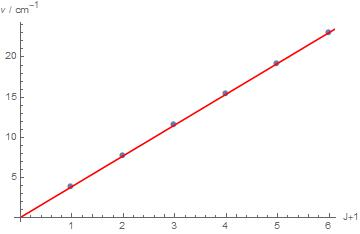
\includegraphics[width=0.5\linewidth]{chap13-18.jpg}
\end{figure}
and thus
\begin{align}
2\tilde{B} &= \SI{3.845}{cm^{-1}}\\
-4\tilde{D} &= \SI{-2.555e-5}{cm^{-1}}
\end{align}
i.e.
\begin{align}
\tilde{B} &= \SI{1.923}{cm^{-1}}\\
\tilde{D} &= \SI{6.388e-6}{cm^{-1}}
\end{align}

\ex{32}
Since
\begin{equation}\label{key}
\tilde{\nu}_{\text{obs}} = \tilde{T}_e + \qty(\dfrac{1}{2}\tilde{\nu}_e' - \dfrac{1}{4}\tilde{x}_e'\tilde{\nu}_e') - \qty(\dfrac{1}{2}\tilde{\nu}_e'' - \dfrac{1}{4}\tilde{x}_e''\tilde{\nu}_e'') + \qty(\tilde{\nu}_e' - \tilde{x}_e'\tilde{\nu}_e')v' - \tilde{x}_e'\tilde{\nu}_e'v'^2
\end{equation}
Rewrite that as
\begin{equation}\label{key}
\tilde{\nu}_{\text{obs}}(v') = A + Bv' + Cv'^2
\end{equation}
thus we can fit the data as
\begin{figure}[H]
	\centering
	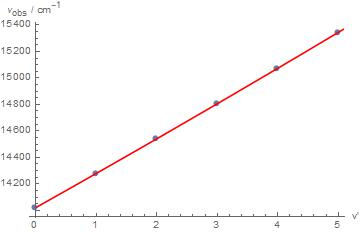
\includegraphics[width=0.5\linewidth]{chap13-32.jpg}
\end{figure}
and
\begin{equation}\label{key}
\tilde{\nu}_{\text{obs}}(v') = 14020.1 + 257.114 v' + 1.57143 v'^2
\end{equation}
thus
\begin{align}
(\tilde{\nu}_e' - \tilde{x}_e'\tilde{\nu}_e') &= \SI{257.114}{cm^{-1}}\\
\tilde{x}_e'\tilde{\nu}_e' &= \SI{-1.57143}{cm^{-1}}
\end{align}
i.e.
\begin{align}
\tilde{\nu}_e' &= \SI{255.542}{cm^{-1}}\\
\tilde{x}_e'\tilde{\nu}_e' &= \SI{-1.571}{cm^{-1}}
\end{align}

\ex{37}
\begin{align}
I_{xx} &= \sum_j m_j y_j^2 = m + 2m\sin^2 30\textdegree = \dfrac{3}{2}m\\
I_{yy} &= \sum_j m_j x_j^2 = 0 + 2m\cos^2 30\textdegree = \dfrac{3}{2}m\\
I_{zz} &= \sum_j m_j( x_j^2 + y_j^2) = m + m + m = 3m
\end{align}

\ex{40}
Eq 13.55 reads
\begin{equation}\label{key}
a_2(t) \approx (\mu_z)_{12}E_{0z}\qty[\dfrac{1 - \e^{\I(E_2-E_1+h\nu)t/\hbar}}{E_2 - E_1 + h\nu} + \dfrac{1 - \e^{\I(E_2-E_1-h\nu)t/\hbar}}{E_2 - E_1 - h\nu}]
\end{equation}
The second term dominates when $ E_2 - E_1 \approx h\nu $, thus
\begin{align}
a_2(t) &\approx \dfrac{1 - \e^{\I(E_2-E_1-h\nu)t/\hbar}}{E_2 - E_1 - h\nu}\\
a_2(t)^* &\approx \dfrac{1 - \e^{-\I(E_2-E_1-h\nu)t/\hbar}}{E_2 - E_1 - h\nu}
\end{align}
$ \therefore $
\begin{align}
a_2^*(t)a_2(t) &\approx \dfrac{1 - \e^{\I(E_2-E_1-h\nu)t/\hbar} - \e^{-\I(E_2-E_1-h\nu)t/\hbar} + 1}{(E_2 - E_1 - h\nu)^2}\notag\\
&\approx \dfrac{2 - 2\cos\dfrac{(E_2-E_1-h\nu)t}{\hbar}}{(E_2 - E_1 - h\nu)^2}\notag\\
&\approx \dfrac{\sin^2\dfrac{(E_2-E_1-h\nu)t}{2\hbar}}{(E_2 - E_1 - h\nu)^2} \notag\\
&\approx \dfrac{\sin^2\dfrac{(E_2-E_1-\hbar\omega)t}{2\hbar}}{(E_2 - E_1 - \hbar\omega)^2} 
\end{align}

\ex{43}
\begin{align}
I_{0\ra 1} &\approx \intdinf \psi_1(\xi)\xi\psi_0(\xi) = \sqrt{\dfrac{2a}{\pi}}\intdinf \xi^2 \e^{-\xi^2}\dd\xi \notag\\
&= \sqrt{\dfrac{2\alpha}{\pi}} \dfrac{\sqrt{\pi}}{2} \notag\\
&= \sqrt{\dfrac{\alpha}{2}} 
\end{align}
\begin{align}
I_{1\ra 2} &\approx \intdinf \psi_2(\xi)\xi\psi_1(\xi) = \sqrt{\dfrac{a}{\pi}}\intdinf \xi^2(2\xi^2 - 1) \e^{-\xi^2}\dd\xi \notag\\
&= \sqrt{\dfrac{\alpha}{\pi}} \sqrt{\pi} \notag\\
&= \sqrt{\alpha}
\end{align}
thus
\begin{equation}\label{key}
\dfrac{I_{0\ra 1}}{I_{1\ra 2}} = \dfrac{1}{\sqrt{2}}
\end{equation}

\ex{45}
$ \ce{CH_2Cl_2} $ belongs to $ C_{2v} $ group, thus
\begin{table}[H]
	\begin{tabular}{c|cccc}
		   & $ \hat{E} $ & $ \hat{C}_2 $ & $ \hat\sigma_v $ & $ \hat\sigma_v' $\\ \hline
		$ \Gamma $ & 15 & -1 & 3 & 3
	\end{tabular}
\end{table}
\begin{align}
a_{A_1} &= \dfrac{1}{4}(15 - 1 + 3 + 3) = 5\\
a_{A_2} &= \dfrac{1}{4}(15 - 1 - 3 - 3) = 2\\
a_{B_1} &= \dfrac{1}{4}(15 + 1 + 3 - 3) = 4\\
a_{B_2} &= \dfrac{1}{4}(15 + 1 - 3 + 3) = 4
\end{align}
$ \therefore $
\begin{equation}\label{key}
\Gamma_{3N} = 5A_1 + 2A_2 + 4B_1 + 4B_2
\end{equation}
Since 
\begin{align}
\Gamma_{\text{trans}} &= A_1 + B_1 + B_2\\
\Gamma_{\text{rot}} &= A_2 + B_1 + B_2 
\end{align}
we have
\begin{equation}\label{key}
\Gamma_{\text{vib}} = 4A_1 + A_2 + 2B_1 + 2B_2
\end{equation}
and the $ A_2 $ vibrational mode is infrared inactive and the others are infrared active.

\ex{51}


\end{document}